\documentclass[10pt]{article}
\usepackage[margin=0.7in]{geometry}
\usepackage[T1]{fontenc}
\usepackage{graphicx,hyperref}
\begin{document}
\sloppy
\section*{Independent review of mutable signed-graph find}
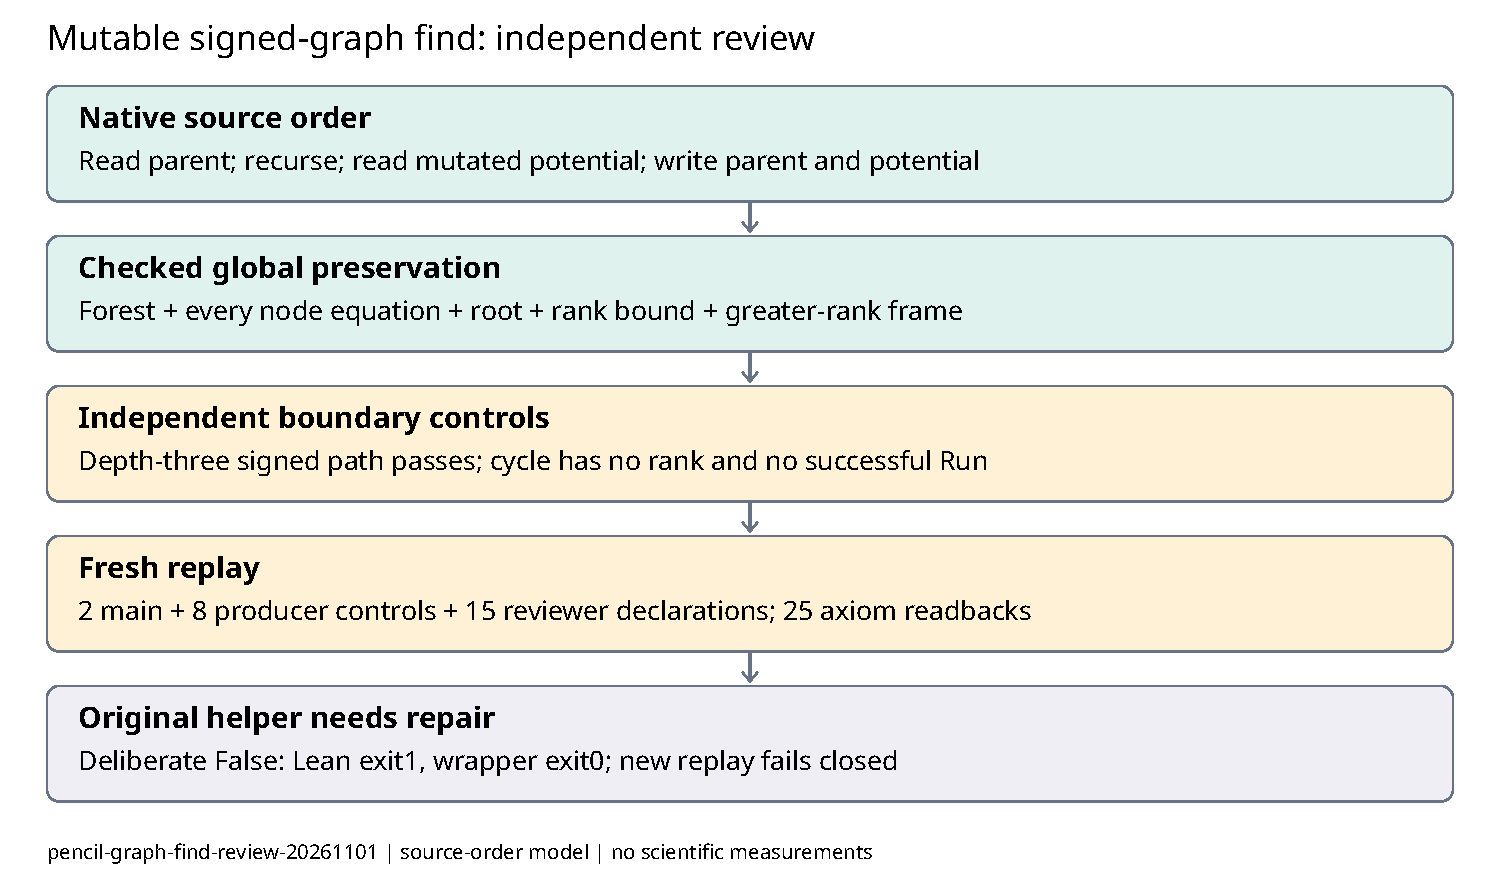
\includegraphics[width=\linewidth]{flow.pdf}
The two mutable-find theorems replay successfully from the published source bytes. Eight producer controls and fifteen reviewer declarations also pass. Twenty-five named axiom readbacks contain only permitted axioms. The mathematical result and the source-order correspondence are validated at the stated finite functional-heap scope. The original producer check.py has a demonstrated failure-propagation defect; workflow completion requires a separately published and reviewed repair.\par\medskip
Bound inputs and independence. Producer head60346e7f2b831aa88f89d7967b9e74e21220422c is the supplied PR3056 head. Find.lean, Controls.lean and Readback.lean were extracted from its state-and-repair-closure/graph-find archive and match the private producer files byte-for-byte. All33 entries in the private producer manifest match. The coordinator's prospective plan is commit6f7a9eec4f4920c3d6267892b906e761a186229c, joint graph-find. Native three\_leads.rs1580-1596 was read before Find.lean. The local PLAN.md execution note was written after reading the producer proof and controls and is explicitly not a prospective plan. This reviewer authored the imported GraphAlgebra component, but did not author Find.lean; this is independent review of the new mutable-state proof, not fully blind re-derivation of all dependencies.\par\medskip
Source-first derivation. Native find increments the operation counter, reads parent[x], returns identity if it is x, otherwise recursively finds that parent, then reads pot[x] from the mutated state, composes, writes parent[x] and pot[x], and returns. Run.step preserves this crucial post-recursion read as t.pot x. Its two simultaneous functional writes express the final array state; the counter and intermediate write observability are outside this model. The strong rank frame establishes that the recursive call leaves the caller's node unchanged because parent rank is strictly lower. Thus no pre-recursion read is silently substituted for a post-recursion read.\par\medskip
The invariant is global. Represents quantifies over every finite node at fixed scalar k and values v. run\_preserves returns the updated Forest, updated Represents, self-parent returned root, evaluated potential semantics, root-rank bound, and a frame for every node with greater rank than the queried node. When x is compressed, its equation follows by affine composition; every other node's equation persists. Strict root-rank decrease shows root is not x, so the update cannot destroy root self-parenthood. The immutable rank witness is an initial acyclicity condition, not an assumed output invariant. run\_exists constructs a finite Run by strong induction on that rank without assuming a preexisting successful trace.\par\medskip
Independent controls. A five-node ZMod17 fixture has path3->2->1->0 and unrelated root4, with edges(-1,2,3), (+1,5,-2), (-1,-4,6). At k=2 and root value7 the three path values are1,2,6; compression yields potential(+1,-11,5). Controls instantiate the actual three-level Run, global representation and forest preservation, all three parent writes, the post-recursion child frame, and the unrelated-node frame. Replacing signed composition by unsigned arithmetic gives the wrong value; resetting potentials breaks representation. A two-node cycle has no possible decreasing Nat rank, no root, and no successful Run. A separate theorem proves every Run requires an initial root. These checks establish satisfiable forest premises and an explicit failure boundary. There is no fuel parameter in this model, so insufficient-fuel behavior is not claimed or tested; native stack capacity remains outside the termination theorem.\par\medskip
Machine verification. Fresh private replay compiled GraphAlgebra, Find, Controls, Reviewer, Readback and ReviewerReadback. The main preservation theorem reads back only propext; run\_exists has no axioms. The other named readbacks use only propext and Quot.sound. Each final gate returned zero with unchanged source/helper/direct-olean bindings. The private snapshot includes dependency source/olean files from the prior stable graph snapshot; GraphAlgebra was freshly rebuilt. Transitive Mathlib cache binaries and the compiler retain their usual trust boundary; no independent binary kernel rechecker was run. The first dependency attempt lacked Product in its path; it was corrected by copying the stable dependency snapshot. Reviewer attempt1 needed explicit constructor equality and corrected induction binder names; its failed source and logs are retained.\par\medskip
Producer gate defect. The original helper records a Lean exit\_code, breaks on nonzero, asserts unchanged bindings, then exits normally. In a fresh negative-control directory, its exact helper bytes were run against example : False := by trivial. Lean returned1 and reported an unsolved False goal, while the Python process returned0. This is a controlled demonstration of the helper defect, not an accepted theorem or a failure of the reviewed mathematics. The fresh reviewer helper propagates compiler failures and binding failures; its passing checks support the scoped mathematical result. Coordinator has requested a separate repair packet; this review does not mark the original workflow complete.\par\medskip
Concrete boundaries. State uses Fin n indices and arbitrary commutative-ring coefficients, not native Vec indexing, i8 signs, canonical scalar words, counters, or compiled Rust. Initial forest and representation assumptions are explicit. This packet does not establish node creation/union preservation of those assumptions, fixed-anchor metadata, native stack capacity, or group-to-scalar interpretation. The reviewed claim is preservation and existence for mutable find in the source-order model; it is not a proof of all SignedGraph operations.\par\medskip
Review results. Machine status: passed for the two main theorems, eight producer controls and fifteen independent declarations. Source fidelity: faithful\_scoped for the finite functional-heap find relation and stated invariants. Mathematical review outcome: validated\_scoped. Original helper workflow outcome: needs\_revision because nonzero compiler exits are not propagated. No scientific trials, cohort runs, performance measurements or repository modifications occurred.\par\medskip
\end{document}